\chapter{InstructGPT and DeepSeek-R1-Style Training}

Chapter 11 built RLHF from a language-model policy $\pi_\theta$, a reward model $r_\phi$, a frozen reference $\pi_{\mathrm{ref}}$, and the updates RLOO and PPO. The policy loop in that chapter samples a reply $y$ from $\pi_\theta$, scores it with $r_\phi$, and steps $\theta$. That loop already assumes a starting $\pi_\theta$ and a frozen $\pi_{\mathrm{ref}}$: both are a copy of a supervised checkpoint, trained on fixed demo pairs before any preference data are used. Chapter 11 did not derive that supervised step.

This chapter does. It derives \textbf{supervised fine-tuning (SFT)} --- the procedure that produces that checkpoint --- and, when the answer \textit{is} checkable, replaces $r_\phi$ by a fixed \textbf{program}. Those pieces are then used in InstructGPT and in DeepSeek-R1-style training. Neither is a new kind of policy gradient.

\textbf{InstructGPT} (\citetxt{ouyang2022}{Ouyang et al., 2022}) uses SFT on human-written demo pairs $(x,y)$. From a pretrained checkpoint it raises the probability of those replies. The resulting weights initialize $\pi_\theta$ and are frozen as $\pi_{\mathrm{ref}}$. Preference comparisons then train $r_\phi$, and the policy loop of Chapter 11 improves $\pi_\theta$.

When a program can score $y$, the same policy-gradient loop no longer needs a reward model $r_\phi$. \citetxt{deepseek2025}{Guo et al.\ (2025)} published two systems of that kind. \textbf{DeepSeek-R1-Zero} applies \textbf{group relative policy optimization (GRPO)} to the base model with a rule verifier and no SFT. \textbf{DeepSeek-R1} begins with a small cold-start SFT, applies GRPO, clones only traces that pass a hard filter, applies GRPO a second time, then SFT smaller dense models on those kept traces. For one prompt, GRPO samples a \textbf{group} of replies, turns those group scores into advantages, and clips the importance ratio as PPO does. Each reply in those GRPO stages is scored by a \textbf{verifier}: a fixed program that checks the final answer and the format, not a reward model $r_\phi$.

We are not training those published systems (InstructGPT and DeepSeek-R1) in this chapter --- not their base models, data, or infrastructure. The rest of this chapter derives SFT, the program score, GRPO, and rejection sampling, and uses a pipeline of the same shape on the Chapter 11 toy. That toy already has checkable answers, so a program can score $y$. Section 12.1 is SFT, used by both. Section 12.2 is InstructGPT (that SFT plus Chapter 11's RLHF). Section 12.3 is the DeepSeek-R1-style group: rule reward, GRPO, and reject then SFT.

\section{Supervised fine-tuning}

SFT starts from a pretrained checkpoint $\pi_{\mathrm{base}}$ and a dataset of \textbf{fixed} prompt--reply pairs \[
\mathcal{D}_{\mathrm{SFT}}=\bigl\{(x^{(n)}, y^{(n)})\bigr\}_{n=1}^{N}.
\] The replies are written (or already accepted) strings --- human demos in InstructGPT, long chain-of-thought traces in a DeepSeek-R1-style cold start. The goal is to raise the probability of those strings: maximize $\pi_\theta(y\mid x)$ on $\mathcal{D}_{\mathrm{SFT}}$. There is no sampler and no reward.

On one training pair $(x,y)$ with $y=(y_1,\ldots,y_T)$, \[
\log\pi_\theta(y\mid x)
=
\sum_{t=0}^{T-1}
\log\pi_\theta(y_{t+1}\mid x, y_1,\ldots,y_t).
\] The statistical target is the \textbf{total} log-likelihood of the dataset \begin{equation}
J_{\mathrm{SFT}}(\theta)
=
\sum_{n=1}^{N}
\log\pi_\theta\bigl(y^{(n)}\mid x^{(n)}\bigr).
\tag{12.1}
\end{equation} \begin{equation}
L_{\mathrm{SFT}}(\theta)
=
-\frac1N J_{\mathrm{SFT}}(\theta).
\tag{12.2}
\end{equation}

In ordinary autoregressive generation the prefix $y_1,\ldots,y_t$ is sampled from the model's previous outputs: $y_1\sim\pi_\theta(\cdot\mid x)$, then $y_2\sim\pi_\theta(\cdot\mid x,y_1)$, and so on.

\textbf{Teacher forcing} does not use those samples. For the SFT loss, each term $\log\pi_\theta(y_{t+1}\mid x, y_1,\ldots,y_t)$ uses the \textbf{gold} prefix $y_1,\ldots,y_t$ from $\mathcal{D}_{\mathrm{SFT}}$, and the target is gold $y_{t+1}$. If the gold sentence is ``The cat sat'' and the model predicts \texttt{dog} instead of \texttt{cat}, training still feeds gold \textbf{\texttt{cat}} as the next input and applies a loss against gold \texttt{sat}. At inference, \texttt{dog} would be fed and the rest of the string would drift. Teacher forcing is that training setup --- not a second teacher network.

Differentiating (12.2) gives \begin{equation}
\nabla_\theta L_{\mathrm{SFT}}(\theta)
=
-\frac1N\sum_{n=1}^{N}
\sum_{t=0}^{T_n-1}
\nabla_\theta\log\pi_\theta\bigl(y^{(n)}_{t+1}\mid x^{(n)}, y^{(n)}_1,\ldots,y^{(n)}_t\bigr).
\tag{12.3}
\end{equation} Gradient descent with step size $\alpha>0$ is \begin{equation}
\theta\leftarrow\theta-\alpha\,\nabla_\theta L_{\mathrm{SFT}}(\theta).
\tag{12.4}
\end{equation} In practice: a mini-batch forward, $L_{\mathrm{SFT}}$, \texttt{backward}, optimizer step.

After enough steps, $\pi_\theta(y\mid x)$ is larger than it was under $\pi_{\mathrm{base}}$ on the demos. That is \textbf{behavioral cloning} of fixed strings. SFT does not sample its own replies, does not call a verifier, and does not optimize ``any correct trace'' --- only the traces in $\mathcal{D}_{\mathrm{SFT}}$. The model is also biased toward gold prefixes; at use time the prefix is its \textbf{own} tokens (exposure bias). Sampling scored by a reward is what closes that gap (Sections 11.5--11.6 and 12.3.2).

\begin{implnote}[Algorithm (SFT)]
\textbf{Input:} pretrained $\pi_{\mathrm{base}}$; $\mathcal{D}_{\mathrm{SFT}}=\{(x^{(n)},y^{(n)})\}$; step size $\alpha$; epochs $E$. \textbf{Output:} fine-tuned $\pi_\theta$.

\begin{enumerate}
\item Set $\theta\leftarrow\theta_{\mathrm{base}}$.
\item For epoch $=1,\ldots,E$, for each mini-batch $B\subset\mathcal{D}_{\mathrm{SFT}}$:
\begin{itemize}
\item Form $L_{\mathrm{SFT}}$ on $B$.
\item $\theta\leftarrow\theta-\alpha\nabla_\theta L_{\mathrm{SFT}}$.
\end{itemize}
\item Return $\pi_\theta$.
\end{enumerate}

\end{implnote}

We use \texttt{log\_pi} and \texttt{make\_h} from Section 11.5. On a gold pair, \texttt{log\_pi(h, x, y)} \textbf{is} teacher forcing: each term conditions on the gold prefix $y_{:t}$.

\lstinputlisting{../code/ch12/sft.py}


\section{InstructGPT: SFT then RLHF}

\textbf{InstructGPT} (\citetxt{ouyang2022}{Ouyang et al., 2022}) begins with SFT on human demo pairs, as in Section 12.1. The resulting checkpoint initializes $\pi_\theta$ and is frozen as $\pi_{\mathrm{ref}}$, which is the reference already used in Section 11.4. Chapter 11's reward model and policy loop follow.

\textbf{Stage 0 (SFT, once).} Humans write demo pairs $(x,y)$. Run the SFT algorithm from $\pi_{\mathrm{base}}$. The resulting checkpoint is $\pi_\theta$. A frozen copy is $\pi_{\mathrm{ref}}$.

\textbf{Stage 1 (reward model, once).} After SFT, a \textbf{prompt set} $\mathcal{D}$ is used: queries $x$ only, no gold replies. For each prompt, several replies are sampled from the SFT policy. A human marks a preferred reply $y_w$ and a rejected reply $y_l$. Those triples train $r_\phi$ as in (11.3); then $\phi$ is frozen.

\textbf{Stage 2 (policy loop).} The same prompt set is used again. A prompt $x$ is drawn from $\mathcal{D}$, a reply $y$ is sampled from the \textbf{current} $\pi_\theta$, and the score is $R=r_\phi(x,y)-\beta\,\mathrm{KL}$ as in (11.4). PPO clips and updates $\theta$ as in Section 11.6, then a new batch is sampled. $\pi_{\mathrm{ref}}$ never samples.

\begin{figure}[ht]
\centering
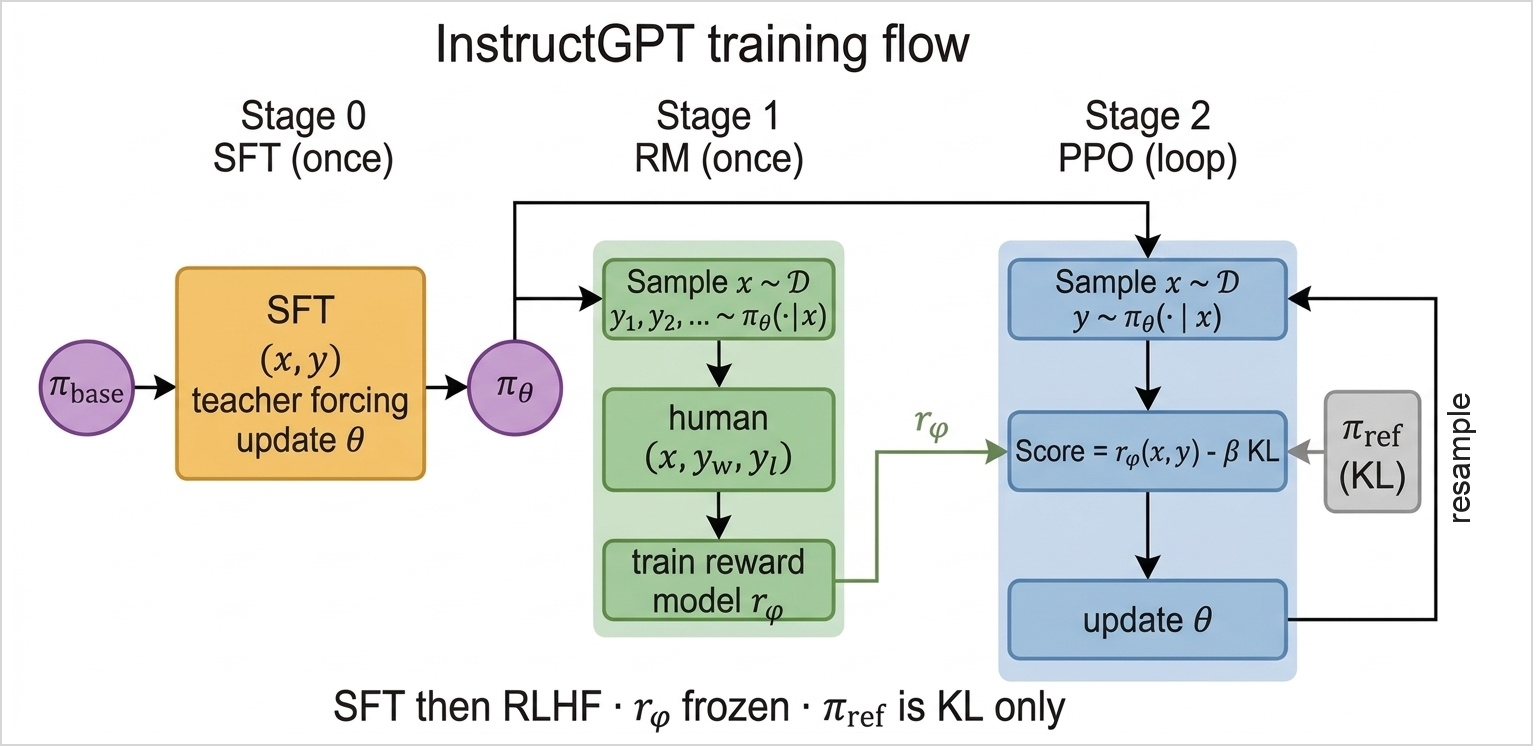
\includegraphics[width=0.85\textwidth]{instructgpt_style_flow.jpg}
\caption{InstructGPT: SFT, reward model, then PPO.}\label{fig-15-1}
\end{figure}

That is the same math as Chapter 11. SFT is (12.1)--(12.4); it produces the frozen $\pi_{\mathrm{ref}}$.

\section{DeepSeek-R1-style training}

Section 12.2 needs humans (or $r_\phi$ trained from humans) because a chat reply has no gold answer to check. When $y$ \textit{is} checkable, a program scores the reply. \textbf{DeepSeek-R1-Zero} is GRPO from $\pi_{\mathrm{base}}$ with no SFT. \textbf{DeepSeek-R1} (and the toy here) uses SFT (Section 12.1) as a cold start, then the chain below:

\begin{figure}[ht]
\centering
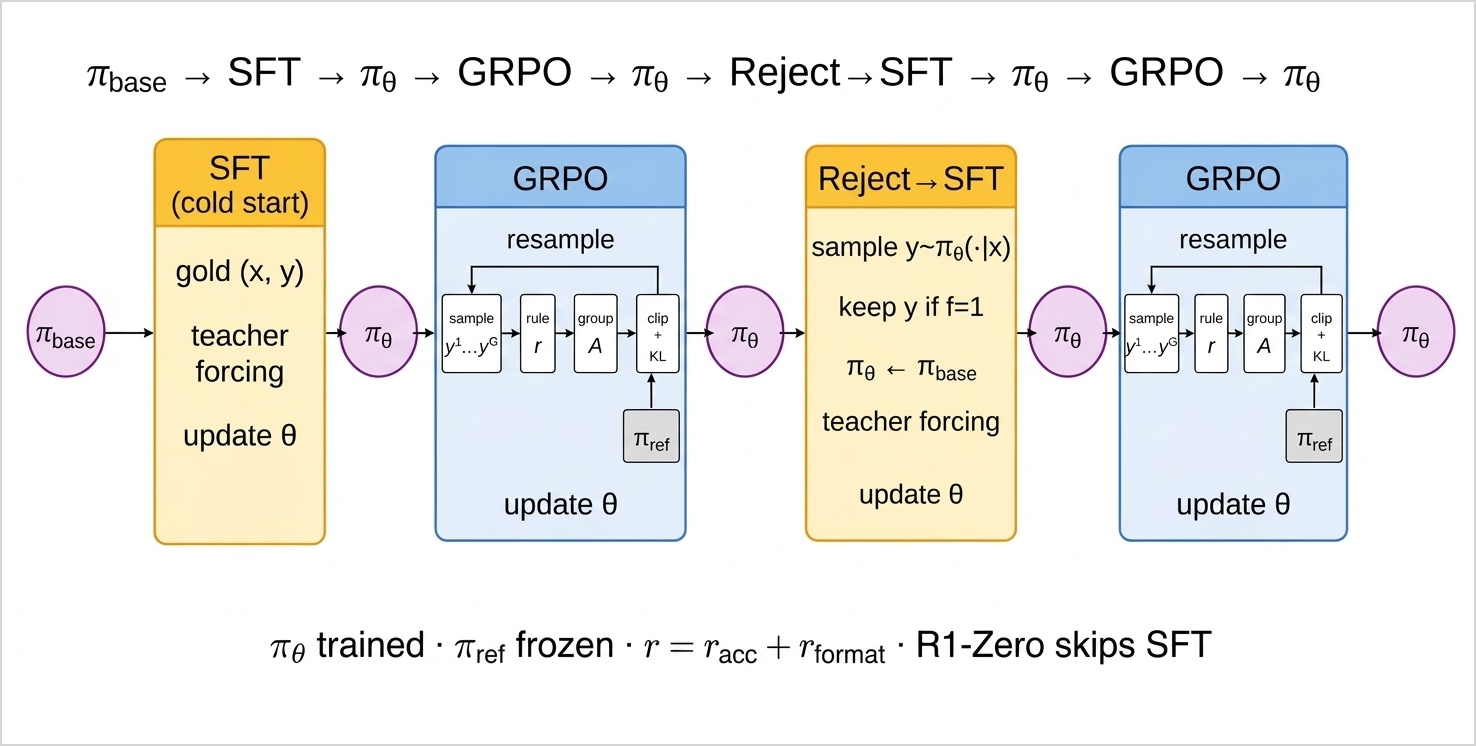
\includegraphics[width=0.90\textwidth]{deepseek_r1_style_flow.jpg}
\caption{DeepSeek-R1-style training: SFT, GRPO, reject then SFT, GRPO.}\label{fig-15-2}
\end{figure}

GRPO is derived in Section 12.3.2; reject-then-SFT in Section 12.3.3. The second GRPO freezes a \textbf{new} $\pi_{\mathrm{ref}}$ at the start of that stage. Distillation is not a box on that chain: it runs SFT on a smaller student. DeepSeek-R1 uses the kept traces from Reject→SFT for that SFT.

\subsection{Rule-based reward}

Math, code with unit tests, and short-answer STEM have a key: a gold number, a test suite, or a short target string. A fixed \textbf{verifier}, usually a program that implements rules instead of a reward model $r_\phi$, scores each reply. That reward is an \textbf{accuracy} term plus a \textbf{format} term: \begin{equation}
r(x,y)=r_{\mathrm{acc}}(x,y)+r_{\mathrm{format}}(y).
\tag{12.5}
\end{equation} No $\phi$ is trained, and humans do not label each sampled $y$. Each prompt $x$ in $\mathcal{D}$ is stored with a \textbf{key} the policy does not see --- a gold answer or unit tests --- and the verifier uses that key to score $y$. The two terms in (12.5) are $0$--$1$ checkers:

\begin{itemize}
\item $r_{\mathrm{format}}(y)\in\{0,1\}$: $1$ if the reply has the required format (for example \texttt{<think>…</think>} tags).
\item $r_{\mathrm{acc}}(x,y)\in\{0,1\}$: $1$ if the extracted answer matches the key. Math: take only a specified slot such as \texttt{\textbackslash\{\}boxed\{…\}} and match gold (numbers as numbers; expressions with a computer-algebra check). Code: run tests. If that slot is missing, $r_{\mathrm{acc}}=0$ even when the digits appear in prose. The chain of thought is not scored.
\end{itemize}
Adding them gives $r\in\{0,1,2\}$. For example, take $x=$ \texttt{2+2} with gold $4$. A tagged reply with \texttt{\textbackslash\{\}boxed\{4\}} scores $r=2$; tagged with \texttt{\textbackslash\{\}boxed\{5\}} scores $r=1$; untagged \texttt{the answer is 4} scores $r=0$ if $r_{\mathrm{acc}}$ looks only in the boxed slot.

Those scores are a design choice. If $r_{\mathrm{acc}}$ also accepts the number in prose, the same untagged reply \texttt{the answer is 4} scores $r=1$.

The RL \textbf{loop} is the same shape as Chapter 11 Stage 2: sample $y$ from $\pi_\theta$, score, update $\theta$, resample, KL to a frozen $\pi_{\mathrm{ref}}$. The score is now (12.5) instead of $r_\phi$, and the advantage is formed as in Section 12.3.2. Leave $r_\phi$ out of (12.5): this stage is scored by the program only.

\subsection{GRPO}

\textbf{GRPO} (Group Relative Policy Optimization) was introduced in DeepSeekMath (\citetxt{shao2024}{Shao et al., 2024}): for one prompt, sample a \textbf{group} of replies, turn those group scores into advantages, and apply a PPO-style clip. DeepSeek-R1-Zero then used that update with a \textbf{rule} reward from the base model (no SFT). DeepSeek-R1 uses the same update after a cold-start SFT, and again after reject-then-SFT (\citetxt{deepseek2025}{Guo et al., 2025}).

We do not implement those papers' models or training stack. We follow a similar update on the Chapter 11 toy. The toy already has a gold key, so a program can score $y$ and we skip $r_\phi$ (Section 12.3.1). Section 11.6 already forms $A_k$ from \textbf{other replies to the same} $x$ (leave-one-out). GRPO is that idea with a group mean and std.

Fix one prompt $x\in\mathcal{D}$ with a key. Copy $\theta_{\mathrm{old}}\leftarrow\theta$. \textbf{Sample} a group of $G$ replies, i.i.d. given that same $x$: \[
y^{(1)},\ldots,y^{(G)}\sim\pi_{\theta_{\mathrm{old}}}(\cdot\mid x),
\qquad
y^{(i)}=\bigl(y^{(i)}_1,\ldots,y^{(i)}_{T_i}\bigr).
\] The sampling condition is only $x$: reply $i$ does not see the other replies. As in (11.1), each $y^{(i)}$ is generated with \[
\pi_{\theta_{\mathrm{old}}}\bigl(y^{(i)}\mid x\bigr)
=
\prod_{t=0}^{T_i-1}
\pi_{\theta_{\mathrm{old}}}\bigl(y^{(i)}_{t+1}\mid x,y^{(i)}_1,\ldots,y^{(i)}_t\bigr).
\]

Score each finished reply with (12.5): $r_i=r_{\mathrm{acc}}\bigl(x,y^{(i)}\bigr)+r_{\mathrm{format}}\bigl(y^{(i)}\bigr)$.

\textbf{Group advantage.} Baseline is this group's own mean, then scale by the group's std so $A$ is order-1 when $r$ is $0/1/2$: \begin{equation}
A_i
=
\frac{r_i-\mathrm{mean}(r)}{\mathrm{std}(r)+\delta}.
\tag{12.6}
\end{equation} $\delta>0$ is a small constant added so we never divide by zero (typical $10^{-8}$). If every $r_i$ is equal, then $\mathrm{mean}(r)=r_i$ as well, so the numerator is $0$ and $\mathrm{std}(r)=0$. Without $\delta$ that is $0/0$ (undefined), not a blow-up. With $\delta$ you get $A_i=0/\delta=0$ --- no update (the group has nothing to prefer). There is no ``nonzero numerator over zero std'' case: $\mathrm{std}(r)=0$ if and only if every $r_i$ is the same, which forces the numerator to $0$ too. Section 11.6 uses $A_k=R_k-b_k$ with leave-one-out $b_k$. Here the baseline is the group's mean of the $G$ rule scores; the std only rescales.

\begin{asidenote}[Note]
\textbf{Toy} ($G=4$, $x=$ \texttt{2+2}). Say $r=(2,1,0,1)$. Then $\mathrm{mean}=1$, $\mathrm{std}=\sqrt{1/2}$, so $A\approx(1.41,\;0,\;-1.41,\;0)$. The $r=2$ reply is pushed up; the $r=0$ reply is pushed down; the two $r=1$ replies sit at $0$.

\end{asidenote}

The importance ratio remains the same as in (11.8): \[
\rho_i(\theta)
=
\frac{\pi_\theta\bigl(y^{(i)}\mid x\bigr)}{\pi_{\theta_{\mathrm{old}}}\bigl(y^{(i)}\mid x\bigr)}.
\] Freeze $A_i$ and minimize the same clip scalar as (11.9), \[
L_{\mathrm{clip}}(\theta)
=
-\frac1G\sum_{i=1}^{G}
\min\bigl(
\rho_i(\theta)\,A_i,\;
\mathrm{clip}(\rho_i(\theta),1-\varepsilon,1+\varepsilon)\,A_i
\bigr).
\] \textbf{KL.} In (11.4) the score $R_\theta$ is $r_\phi-\beta\log(\pi_\theta/\pi_{\mathrm{ref}})$, so the log-ratio goes into $A_k$. Here $r_i$ is only (12.5). Subtracting the KL from $r_i$ would send it through the group mean and std in (12.6), so $A_i$ would mix the rule score with drift from $\pi_{\mathrm{ref}}$. Therefore the KL is added to the loss instead: \begin{equation}
L_{\mathrm{GRPO}}(\theta)
=
L_{\mathrm{clip}}(\theta)
+
\beta\,\mathrm{KL}\bigl(\pi_\theta(\cdot\mid x)\,\|\,\pi_{\mathrm{ref}}(\cdot\mid x)\bigr).
\tag{12.7}
\end{equation} The KL is estimated by averaging over the $G$ sampled replies: \[
\frac1G\sum_{i=1}^{G}
\log\frac{\pi_\theta\bigl(y^{(i)}\mid x\bigr)}{\pi_{\mathrm{ref}}\bigl(y^{(i)}\mid x\bigr)}
\approx
\mathrm{KL}\bigl(\pi_\theta(\cdot\mid x)\,\|\,\pi_{\mathrm{ref}}(\cdot\mid x)\bigr).
\] $\pi_{\mathrm{ref}}$ is a freeze of $\pi_\theta$ \textbf{at the start of this RL stage}. It only enters (12.7). It never samples.

$A_i$ and $\theta_{\mathrm{old}}$ stay frozen on the inner loop of $E$ gradient-descent steps on (12.7). If $E=1$, there is only one step, so $\rho=1$ and the clip does not act. If $E>1$, several steps on the same batch can drive $\pi_\theta$ far from $\pi_{\theta_{\mathrm{old}}}$; the clip in Section 11.6.2 stops that (Issue 2).

\begin{implnote}[Algorithm (GRPO with a rule reward)]
\textbf{Input:} policy $\pi_\theta$; prompt set $\mathcal{D}$ with keys; rule $r(x,y)=r_{\mathrm{acc}}(x,y)+r_{\mathrm{format}}(y)$; group size $G$; inner steps $E$; clip $\varepsilon$; KL weight $\beta$; step size $\alpha$; $\delta>0$. \textbf{Output:} updated $\pi_\theta$. Frozen $\pi_{\mathrm{ref}}$.

\begin{enumerate}
\item $\pi_{\mathrm{ref}}\leftarrow\pi_\theta$ (freeze).
\item Repeat:
\begin{itemize}
\item Sample $x\in\mathcal{D}$. Set $\theta_{\mathrm{old}}\leftarrow\theta$.
\item Sample $y^{(1)},\ldots,y^{(G)}\sim\pi_{\theta_{\mathrm{old}}}(\cdot\mid x)$.
\item For each $i=1,\ldots,G$:
\begin{itemize}
\item $r_i\leftarrow r_{\mathrm{acc}}\bigl(x,y^{(i)}\bigr)+r_{\mathrm{format}}\bigl(y^{(i)}\bigr)$.
\end{itemize}
\item For each $i=1,\ldots,G$:
\begin{itemize}
\item $A_i\leftarrow\bigl(r_i-\mathrm{mean}(r)\bigr)/\bigl(\mathrm{std}(r)+\delta\bigr)$.
\item Store $\log\pi_{\theta_{\mathrm{old}}}\bigl(y^{(i)}\mid x\bigr)$.
\end{itemize}
\item For $e=1,\ldots,E$:
\begin{itemize}
\item Form $\rho_i(\theta)=\pi_\theta\bigl(y^{(i)}\mid x\bigr)/\pi_{\theta_{\mathrm{old}}}\bigl(y^{(i)}\mid x\bigr)$.
\item Descend on $L_{\mathrm{GRPO}}(\theta)=L_{\mathrm{clip}}(\theta)+\beta\,\mathrm{KL}\bigl(\pi_\theta(\cdot\mid x)\,\|\,\pi_{\mathrm{ref}}(\cdot\mid x)\bigr)$, with $A_i$ and $\theta_{\mathrm{old}}$ frozen.
\end{itemize}
\end{itemize}
\item Return $\pi_\theta$.
\end{enumerate}

\end{implnote}

We use \texttt{sample\_response}, \texttt{log\_pi}, and \texttt{make\_h} from Section 11.5. The rule \texttt{r\_rule} is (12.5) on the toy vocabulary: accuracy is the answer token \texttt{4}; format is a first-token habit (\texttt{it}).

\lstinputlisting{../code/ch12/grpo.py}


\subsection{Rejection sampling then SFT}

GRPO learns from its \textbf{own} samples, but a small SFT on \textbf{filtered} traces is still useful: keep only replies that pass a checker, then start from $\pi_{\mathrm{base}}$ and run SFT on those keepers to update $\theta$ (Section 12.1).

The keep-chance is a \textbf{hard filter} $f(x,y)\in\{0,1\}$: $f=1$ only if $r_{\mathrm{acc}}=1$ and $r_{\mathrm{format}}=1$ (optionally also a readability check). Sample $y\sim\pi(\cdot\mid x)$ from the current rollout policy (usually the actor after GRPO). If $f=1$, keep the pair; if $f=0$, drop it. That is the hard-filter special case of \textbf{rejection sampling}, derived in \appref{H}.

\begin{asidenote}[Note]
\textbf{Kept mix.} A kept reply has distribution \[
p(y\mid x)
=
\frac{\pi(y\mid x)\,f(x,y)}{Z(x)},
\qquad
Z(x)=P(f=1\mid x).
\] This is only the closed form of that mix (\appref{H.3}). The algorithm never uses it: it samples from $\pi$ and checks $f$.

\textbf{Toy.} Four replies with $\pi=(0.40,0.10,0.30,0.20)$ and $f=(1,1,0,0)$ give $Z=0.50$ and $p=(0.80,0.20,0,0)$.

\end{asidenote}

Let $\mathcal{D}_{\mathrm{keep}}$ be the kept pairs and $\mathcal{D}_{\mathrm{gen}}$ optional ordinary supervised data (writing, chat) so the SFT does not forget non-reasoning skills. Then $\mathcal{D}_{\mathrm{SFT}}=\mathcal{D}_{\mathrm{keep}}\cup\mathcal{D}_{\mathrm{gen}}$. The GRPO actor is only the \textbf{sampler}. Set $\pi_\theta\leftarrow\pi_{\mathrm{base}}$, then SFT runs as usual (Section 12.1).

\begin{implnote}[Algorithm (reject then SFT)]
\textbf{Input:} rollout $\pi$; prompts $\mathcal{D}$; filter $f\in\{0,1\}$; optional $\mathcal{D}_{\mathrm{gen}}$; $\pi_{\mathrm{base}}$; step size $\alpha$. \textbf{Output:} SFT policy $\pi_\theta$.

\begin{enumerate}
\item $\mathcal{D}_{\mathrm{keep}}\leftarrow\emptyset$.
\item For many $x\in\mathcal{D}$: sample one or more $y\sim\pi(\cdot\mid x)$; if $f(x,y)=1$, add $(x,y)$ to $\mathcal{D}_{\mathrm{keep}}$.
\item $\mathcal{D}_{\mathrm{SFT}}\leftarrow\mathcal{D}_{\mathrm{keep}}\cup\mathcal{D}_{\mathrm{gen}}$.
\item $\pi_\theta\leftarrow\pi_{\mathrm{base}}$.
\item For several epochs, for each mini-batch $B\subset\mathcal{D}_{\mathrm{SFT}}$: form $L_{\mathrm{SFT}}$ on $B$ (teacher forcing); $\theta\leftarrow\theta-\alpha\nabla_\theta L_{\mathrm{SFT}}$.
\item Return $\pi_\theta$.
\end{enumerate}

\end{implnote}

We use \texttt{sample\_response} and \texttt{make\_h} from Section 11.5. \texttt{sft} is that of Section 12.1. On the toy, $f=1$ iff both terms of (12.5) are $1$.

\lstinputlisting{../code/ch12/reject_then_sft.py}


\textbf{Distillation} is the same SFT, on a \textbf{smaller} network. The last $\pi_\theta$ on the chain above (after the second GRPO) is the trained R1-style model. Distillation does not continue that chain: it trains a different student from \textbf{its own} pretrained $\pi_{\mathrm{base}}$ (not a copy of the teacher), by teacher-forcing on a set $\mathcal{D}_{\mathrm{SFT}}$ of teacher traces. In general those traces need not be rejection-sampled: any teacher strings can be the SFT data, and $f$ is optional. DeepSeek-R1 uses the replies \textbf{already kept} in Reject→SFT --- those $y$ with $f=1$, already in $\mathcal{D}_{\mathrm{SFT}}$ --- and does not run a second rejection loop. It runs that SFT on smaller dense models (Qwen, Llama). That student is not updated by GRPO.

\begin{figure}[ht]
\centering
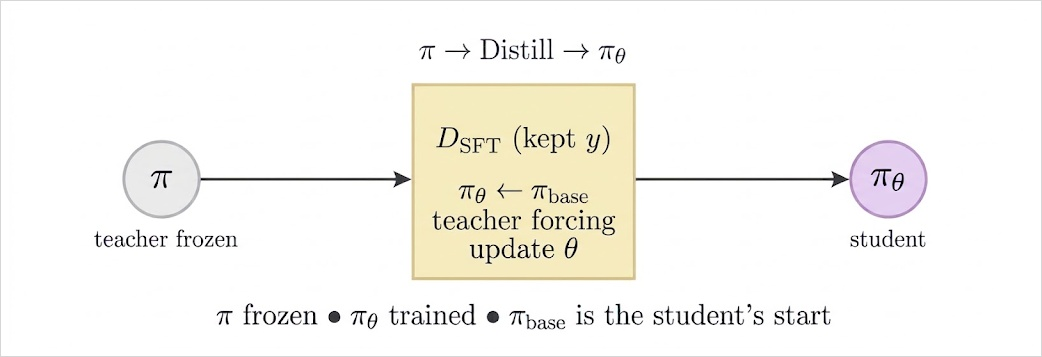
\includegraphics[width=0.70\textwidth]{distillation_flow.jpg}
\caption{Distillation: SFT a smaller student from $\pi_{\mathrm{base}}$ on kept $\mathcal{D}_{\mathrm{SFT}}$.}\label{fig-15-3}
\end{figure}

\begin{implnote}[Algorithm (distillation)]
\textbf{Input:} $\mathcal{D}_{\mathrm{SFT}}$ (teacher traces; here the kept set); student pretrained $\pi_{\mathrm{base}}$ (smaller network); step size $\alpha$. \textbf{Output:} student $\pi_\theta$.

\begin{enumerate}
\item $\pi_\theta\leftarrow\pi_{\mathrm{base}}$ (student; not a copy of the teacher).
\item For several epochs, for each mini-batch $B\subset\mathcal{D}_{\mathrm{SFT}}$: form $L_{\mathrm{SFT}}$ on $B$ (teacher forcing); $\theta\leftarrow\theta-\alpha\nabla_\theta L_{\mathrm{SFT}}$.
\item Return $\pi_\theta$.
\end{enumerate}

\end{implnote}

We use the same \texttt{sft} as Section 12.1. \texttt{d\_sft} is the kept set from reject then SFT above. The student network is a new \texttt{make\_h()} from Section 11.5, not a copy of the teacher.

\lstinputlisting{../code/ch12/distill.py}

